\documentclass[journal,twoside,web]{ieeecolor}
\usepackage{generic}
\usepackage{cite}
\usepackage{amsmath,amssymb,amsfonts}
\usepackage{algorithm}
\usepackage{algpseudocode}
\usepackage{graphicx}
\graphicspath{{./}{../}}
\usepackage{dblfloatfix}
\usepackage{booktabs}
\usepackage{multirow}
\usepackage[table]{xcolor}
\definecolor{black}{rgb}{0,0,0}
\definecolor{blue}{rgb}{0,0,1}
\definecolor{red}{rgb}{1,0,0}
\definecolor{subsectioncolor}{rgb}{0,0,0}
\definecolor{nblue}{rgb}{0,0.263,0.576}
\definecolor{mblue}{rgb}{0.075,0.541,0.855}
\usepackage{array}
\usepackage{makecell}
\usepackage{textcomp}

\usepackage{etoolbox}

\definecolor{myorange}{RGB}{220,90,20}

\makeatletter
\patchcmd{\subsection}{\normalfont}{\normalfont\color{myorange}}{}{}
\makeatother

% \usepackage{xeCJK}
\newcommand{\lmx}[1]{\textcolor{red}{#1}}
\definecolor{tableblue}{RGB}{235, 245, 252}

% ---- Consistent cross-references for IEEE Trans-style templates ----
\newcommand{\figref}[1]{Fig.~\ref{#1}}
\newcommand{\tabref}[1]{Table~\ref{#1}}
\newcommand{\algoref}[1]{Algorithm~\ref{#1}}
\newcommand{\eqnref}[1]{\eqref{#1}} % no leading word, per Trans convention
\newcommand{\secref}[1]{Sec.~\ref{#1}}

\def\BibTeX{{\rm B\kern-.05em{\sc i\kern-.025em b}\kern-.08em
T\kern-.1667em\lower.7ex\hbox{E}\kern-.125emX}}
\markboth{\journalname, VOL. XX, NO. XX, XXXX}
{Li: Efficient and Explainable High-Resolution VQA for Power Inspection}

\makeatletter
\let\NAT@parse\undefined
\makeatother
\usepackage[colorlinks=true, citecolor=blue, linkcolor=blue, urlcolor=blue]{hyperref}

\begin{document}
\title{Efficient and Explainable High-Resolution VQA for Power Inspection with a Domain-Adapted Multimodal Large Language Model}
\author{\centerline{Mingxuan Li, \textit{Member, IEEE}}%
  \thanks{M. Li's ORCID is \href{https://orcid.org/0009-0002-9532-1159}{0009-0002-9532-1159}.}%
}

\maketitle

\begin{abstract}
  Large language models (LLMs) have shown
  exciting potential in powering the growth of many industries,
  yet their adoption in the power electronics (PE) sector is
  hindered by a lack of specialized PE technical expertise
  and challenges in processing PE-specific data. This study
  presents a pioneering approach to establish a multimodal
  LLM tailored for PE design applications, named PE-GPT.
  The methodology involves enhancing PE-GPT with retrieval
  augmented generation from a PE knowledge base, and
  proposes a hybrid framework that integrates an LLM agent
  with metaheuristic algorithms, Model Zoo, and Simulation
  Repository. This enhances its multimodal processing capabilities and enables integration into the existing design
  workflow. The PE-GPT methodology is demonstrated with
  two case studies: modulation design of the dual-active
  bridge (DAB) converter and circuit parameter design of the
  buck converter. PE-GPT demonstrates a 22.2\% increase in
  correctness compared to human experts. Against other
  leading LLMs, PE-GPT shows a 35.6\% improvement in correctness and a 15.4\% enhancement in consistency, reducing
  hallucination. Hardware experiments validate PE-GPT’s multimodal capabilities in optimizing a five-degree-of-freedom
  modulation strategy for the DAB converter. The generalizability of PE-GPT to other PE design applications and
  associated AI ethical considerations are also discussed. This
  research concludes by outlining inspiring future research
  directions, encouraging researchers to expand the boundaries
  of the PE industry and advance toward a more intelligent era
\end{abstract}

\begin{IEEEkeywords}
  Power inspection, multimodal large language model, high-resolution VQA, token selection, explainable AI, retrieval-augmented generation.
\end{IEEEkeywords}

\section{Introduction}
\label{sec:introduction}

\IEEEPARstart{W}{ith} the rapid integration of renewable energy and the continuous evolution toward large-scale, highly interconnected power systems, grid operation has become more dynamic and uncertain, placing higher demands on reliable Operations \& Maintenance (O\&M)~\cite{wang2020achieving}.
Consequently, utilities increasingly rely on data-driven condition awareness and digitalized inspection to ensure secure and stable operation of diverse power equipment.
Recent years have witnessed remarkable strides in task-specific deep learning models for power equipment condition monitoring and inspection. These advancements have been successfully applied across a broad spectrum of physical power apparatus and inspection paradigms, ranging from deep feature modeling for rotating machinery fault diagnosis~\cite{lu2023rotating} to end-to-end visual detection for transmission-line components~\cite{xie2024power} and few-shot recognition in inspection scenarios~\cite{dong2024transmission}. These studies substantiate the capability of deep models in extracting complex representations from inspection imagery, thereby laying a solid data-driven foundation for intelligent power inspection, particularly in modern inspection settings that increasingly rely on high-resolution imagery containing fine-grained visual details.

However, most of these approaches follow a \emph{task-tailored} development paradigm: the model architecture, training objective, and datasets are optimized for a specific task, hindering their reuse and transfer to other inspection tasks and scenarios.
As inspection requirements evolve toward multi-type querying and auditable decision support, this paradigm faces two fundamental limitations.
First, increasingly fine-grained requirements proliferate specialized models, resulting in a fragmented toolchain and high end-to-end costs in data annotation, iterative development, deployment, maintenance, and version management.
Second, task-specific models are typically designed for a narrow input--output format and lack multimodal reasoning and evidence grounding, making it difficult to fuse heterogeneous monitoring information and domain rules into coherent, auditable conclusions and actionable O\&M recommendations.

Foundation models, particularly large language models (LLMs)~\cite{qwennext, guo2025deepseek} and their multimodal variants~\cite{internvl3, wang2026multimodal}, have demonstrated strong capabilities in instruction following, multimodal understanding, and reasoning, enabling a general-purpose and prompt-driven interface for a wide range of downstream tasks in vertical domains such as healthcare~\cite{medllm, medllm2} and finance~\cite{finalllm, finllm2}.
Inspired by these successes, industry practitioners and researchers are increasingly motivated to adapt MLLMs for power systems to alleviate human workload and achieve highly intelligent fault diagnosis~\cite{powerllava, pegpt}. Yet, transitioning from general-purpose interactions to mission-critical power inspection is fraught with obstacles. Directly deploying generic MLLMs remains non-trivial due to the following domain-specific characteristics:
\begin{enumerate}
  \item \textit{Challenge 1 -- Limited power-domain correctness and regulatory compliance.}
    Power O\&M is governed by strict operational regulations and domain-specific criteria such as  equipment structures, defect taxonomies, and handling procedures.
    Generic MLLMs trained on open-domain corpora often lack such grounded expertise, which may lead to non-compliant, non-auditable, or inconsistent conclusions.

  \item \textit{Challenge 2 -- Physical erasure of micro-evidence in image caused by rigid global scaling.}
    To accommodate predefined vision encoders, mainstream MLLMs rigidly resize inputs to a fixed size such as $336\times336$. However, critical defects in 4K power panoramas often occupy $<1\%$ of the image. This naive global downsampling inevitably causes the irreversible physical erasure of such micro-evidence at the input stage, rendering the model fundamentally blind to fine-grained faults regardless of its downstream reasoning capabilities.

  \item \textit{Challenge 3 -- Inefficient processing of high-resolution inspection imagery.}
    Power monitoring images are typically high-resolution with dominant background redundancy, while informative evidence is sparse.
    Naively encoding the full image produces excessive visual tokens, incurring high latency and memory cost and introducing noisy evidence attribution.

\end{enumerate}

To systematically overcome the aforementioned hurdles, we develop \textbf{PowerBrain}, a domain-specialized MLLM framework that harmonizes deployment-oriented evidence mining with robust knowledge grounding.

Specifically, to tackle \textit{Challenge 1}, we perform supervised instruction tuning (SFT) on power-oriented data and integrate citation-grounded retrieval-augmented generation (RAG). By retrieving explicit regulatory snippets, PowerBrain ensures that its diagnostic conclusions are professionally correct and strictly auditable.
To resolve \textit{Challenge 2}, we introduce the \textbf{Adaptive Resolution Escort Paradigm (AREP)}, which utilizes a recall-oriented ROI proposal module to bypass rigid global scaling. Instead of downsampling the entire panorama, AREP actively routes high-resolution perception budgets to critical regions, effectively preventing the irreversible physical erasure of micro-evidence.
Finally, to address \textit{Challenge 3}, we propose \textbf{Coherent Topological Selection (CTS)}---a coverage-aware, instruction-guided token selection strategy that prunes visual redundancy under a fixed budget $K$. Unlike naive pruning, CTS explicitly preserves evidence continuity along elongated power assets, thereby stabilizing reasoning while minimizing computational and memory overhead .
We instantiate the coarse proposal stage with a line-guided prior for transmission-line inspection and further validate PowerBrain's extensibility on non-line tasks, such as disconnect-switch state recognition and meter OCR, via a consistent VQA interface.

The main contributions of this paper are summarized as follows:
\begin{enumerate}
  \item We develop PowerBrain, a domain-adapted MLLM framework tailored for power inspection. By synergizing domain-oriented instruction tuning with citation-grounded knowledge augmentation, it enables unified modeling and auditable reasoning for diverse power VQA tasks.

  \item We propose AREP module to resolve the physical erasure of micro-evidence caused by rigid global scaling. By dynamically routing high-resolution perception budgets to proposed ROIs, it ensures that fine-grained defects are preserved at the input stage, significantly improving the recall of micro-scale faults.

  \item We design CTS module, a coverage-aware token selection strategy that handles the computational inefficiency of high-resolution imagery. Unlike naive pruning, CTS explicitly preserves the spatial continuity and topological structure of thin, elongated assets, thereby stabilizing reasoning while minimizing inference overhead.

  \item We establish a comprehensive evaluation protocol and a high-resolution benchmark derived from real-world power monitoring data. Systematic validation demonstrates that PowerBrain achieves state-of-the-art diagnostic performance while delivering substantial dividends in terms of latency and memory efficiency.
\end{enumerate}

The remainder of this paper is organized as follows.
~\secref{sec:problem} presents the problem formulation and background.
~\secref{sec:method} introduces the proposed PowerBrain framework and its key evidence-mining modules, including AREP and CTS.
~\secref{sec:domain_adapt} describes the domain adaptation and knowledge augmentation strategy.
~\secref{sec:experiments} reports the experimental settings, comparative results, and ablation studies.
Finally, \secref{sec:conclusion} concludes the paper and discusses future work.

\section{Problem Formulation and Preliminaries}
\label{sec:problem}

% \lmx{两个D，在公式里面看不清楚}

\subsection{Overall Objective}
\label{sec:overall_objective}

Power inspection systems often operate under strict deployment constraints,
including limited latency and GPU memory budgets. Consequently, the model
must balance diagnostic accuracy with computational cost.
We model this requirement as learning a query-conditioned multimodal decision function under an inference budget as indicated by Eq.~\eqnref{eq:overall_obj}.
\begin{equation}
  \begin{aligned}
    \min_{\theta,\,\pi\in\Pi}\ \ &
    \mathbb{E}_{(I,q,a^\star)\sim\mathcal{D}}
    \Big[\ell\big(\mathcal{F}_{\theta}(I,q,D;\pi),\,a^\star\big)\Big] \\
    \text{s.t.}\ \ &
    C(\pi; I,q) \le \tau,
  \end{aligned}
  \label{eq:overall_obj}
\end{equation}
where $(I,q,a^\star)\sim\mathcal{D}$ denotes an image--query pair $(I, q)$ with its ground-truth answer $a^\star$ sampled from the data distribution $\mathcal{D}$; $\mathcal{F}_{\theta}$ is a power-domain-adapted MLLM parameterized by $\theta$; and $D$ denotes optional retrieved evidence from a power knowledge corpus such as  regulations, defect criteria, and handling guidelines.

The decision variable $\pi\in\Pi$ represents a deployment-oriented \emph{evidence policy} that controls how visual evidence is generated and selected before being presented to the MLLM.
In this paper, we instantiate $\pi$ with a two-stage strategy consisting of (i) \emph{adaptive-resolution evidence proposal} (AREP) for budget allocation in high-resolution imagery, and (ii) \emph{coverage-aware token selection} (CTS) for query-conditioned evidence selection with continuity preservation.

$C(\pi; I,q)$ denotes a deployment-oriented cost proxy induced by $\pi$
for a given input, such as the number of processed visual tokens,
end-to-end latency, and peak GPU memory usage.
% Under high-resolution inspection imagery, naively encoding the full image produces a long visual token sequence (typically $N\!\propto\! HW/p^2$ for patch size $p$), and the attention-based multimodal fusion in Transformer-style models often scales as $O(N^2)$ in both computation and memory; thus, $\tau$ motivates designing $\pi$ to compress redundant visual tokens while preserving task-critical evidence.

% overview 大图 双栏
\begin{figure*}[t]
  \centering
  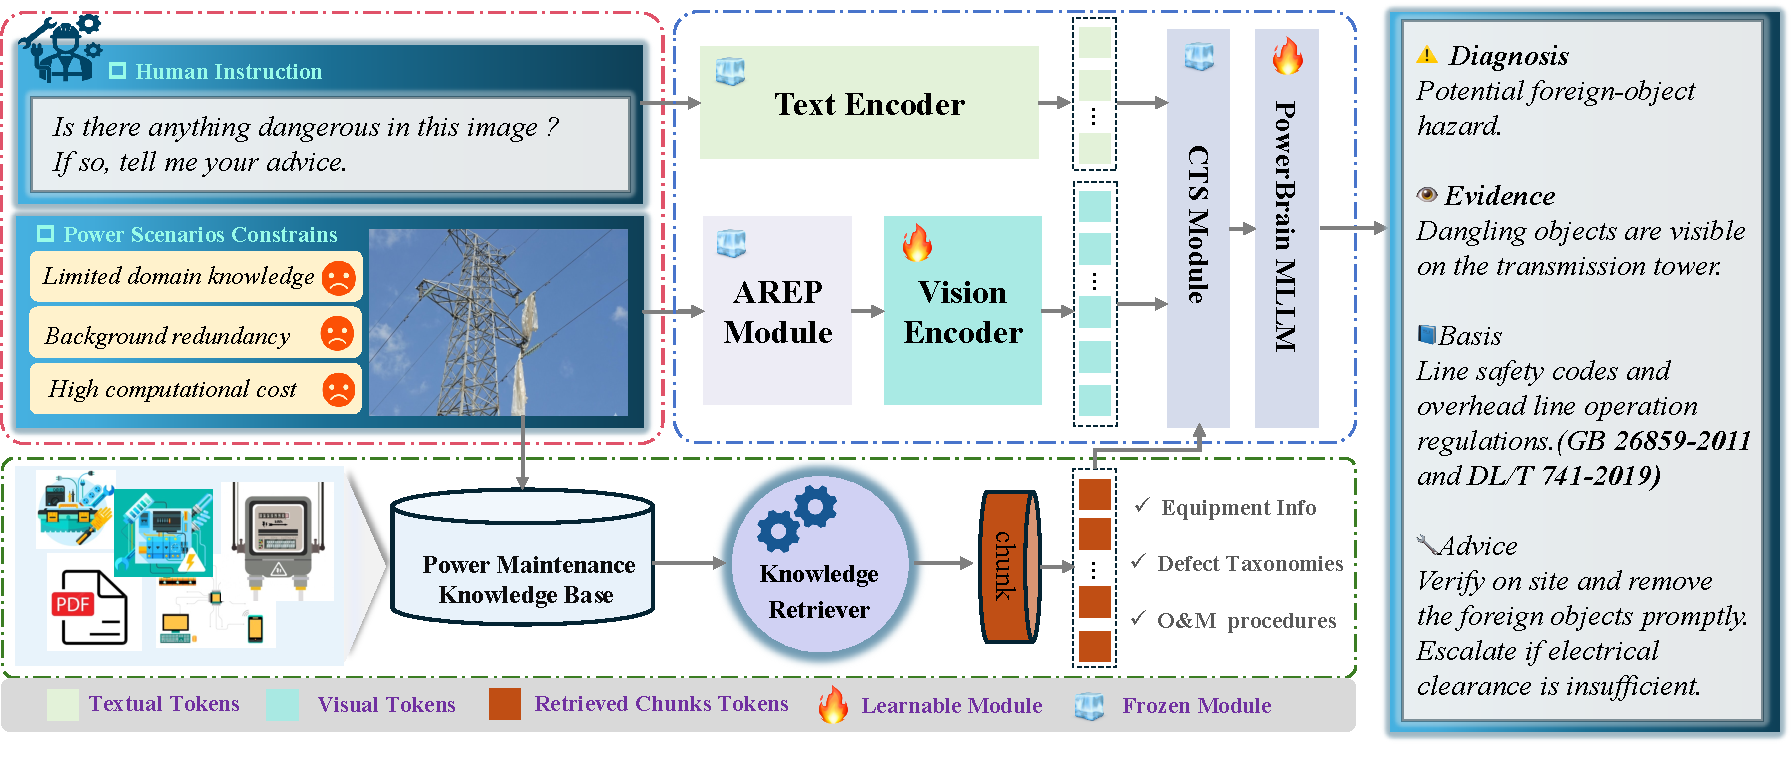
\includegraphics[width=\textwidth]{overview_all.pdf}
  \caption{System overview of PowerBrain for high-resolution power inspection VQA. Given a human instruction and a high-resolution inspection image, the framework addresses three practical challenges, namely limited power-domain knowledge, background redundancy, and high computational cost. On the visual side, the AREP module proposes high-value regions and the CTS module prunes redundant tokens before multimodal reasoning. In parallel, a power-maintenance knowledge base supports citation-grounded retrieval of equipment information, defect taxonomies, and O\&M procedures. The resulting domain-adapted MLLM integrates visual evidence and retrieved knowledge to produce grounded diagnostic responses and actionable maintenance advice.}
  \label{fig:overview}
\end{figure*}

\subsection{Generic Vision-Language Architecture for VQA}
\label{sec:vqa}

We consider a standard multimodal architecture for VQA task consisting of a vision
encoder $\phi(\cdot)$, a vision-language connector $\psi(\cdot)$, and an
autoregressive language decoder $G_\theta(\cdot)$.
Given an image $I$ and a query $q$, the vision encoder extracts a sequence of
visual tokens $V=\phi(I)=\{v_i\}_{i=1}^{N}$, while the query is tokenized as
$T=\mathrm{Tok}(q)=\{t_j\}_{j=1}^{M}$.
The connector aligns and fuses the visual and textual representations to
produce multimodal features $Z=\psi(V,T)$, based on which the decoder
generates the answer $a = G_{\theta}(q,Z)$, corresponding to the conditional
distribution $p_{\theta}(a\mid q,Z)$.

Many connector-decoder architectures also expose query-to-vision attention
patterns that provide a natural signal for identifying question-relevant
visual evidence. Let $A \in \mathbb{R}^{M\times N}$ denote the aggregated
attention from textual tokens to visual tokens, where larger $A_{j,i}$
indicates stronger relevance between $t_j$ and $v_i$. In practice, $A$
can be obtained by averaging attention weights across heads and, when needed,
across upper layers for improved stability.
However, directly applying this generic pipeline to high-resolution power
inspection remains challenging due to several domain-specific constraints,
which are discussed next.

\subsection{Power-Inspection Constraints: Background Redundancy and Evidence Continuity}
\label{sec:power_constraints}

As discussed in~\secref{sec:introduction}, high-resolution power inspection VQA poses two practical constraints.
First, inspection images usually contain large areas of visually uninformative background, whereas fault evidence often occupies only a small portion of the scene.
Directly encoding the full image therefore incurs substantial computational cost while diluting question-relevant cues.
Second, many inspection targets, such as conductors, insulator strings, and equipment boundaries, exhibit elongated or structured spatial layouts.
The evidence relevant to a question is often distributed along these structures rather than concentrated in a compact region, so aggressive relevance-only pruning may fragment critical cues and weaken downstream reasoning.

These characteristics imply that an effective deployment-oriented VQA system should not only reduce redundant visual computation, but also preserve spatially coherent evidence under limited latency and memory budgets.
Consequently, Section~\ref{sec:method} introduces an efficient evidence mining architecture for high-resolution power inspection, while Section~\ref{sec:domain_adapt} further presents domain adaptation and knowledge grounding to improve power-domain correctness and reliability.

\section{Efficient Evidence Mining for High-Resolution Power VQA}
\label{sec:method}

\subsection{Framework Overview}
\label{sec:method_overview}

As illustrated in Fig.~\ref{fig:overview}, we instantiate the evidence policy $\pi$ in Eq.\eqnref{eq:overall_obj} as a coarse-to-fine evidence mining pipeline, to enable budgeted high-resolution VQA for power inspection.
Given an input image $I$ and a query $q$, we first apply \emph{Adaptive Resolution Evidence Proposal} (AREP), $\pi_{\text{are}}$, to allocate visual computation non-uniformly and generate a compact multi-resolution token stream $V_{\text{are}}$ that preserves global context while emphasizing high-information regions.
Then, \emph{Coverage-aware Token Selection} (CTS), $\pi_{\text{cts}}$, uses query-conditioned attention signals to select a budgeted token subset $V_{\pi}$ with $|V_{\pi}|\le K$, while enforcing continuity-aware coverage for structured evidence.
The selected tokens are fed into the MLLM for answer generation, optionally augmented with retrieved domain evidence $D$.
In parallel, the proposal and selection stages preserve spatial evidence that can be visualized as an interpretable trace of the decision process, thereby supporting auditing in practical inspection workflows.

The AREP and CTS modules are detailed in Sec.~\ref{sec:arep} and Sec.~\ref{sec:cts}, respectively.
Domain adaptation and knowledge grounding, including instruction tuning and citation-grounded RAG, are described in Sec.~\ref{sec:domain_adapt}.

% ------------- 这里开始是AREP相关的内容
\subsection{Adaptive Resolution Evidence Proposal (AREP)}
\label{sec:arep}

AREP performs query-agnostic, image-level evidence proposal by allocating high-resolution perception budgets to regions with high estimated information density such as structural or gradient energy on a low-resolution proxy. This importance-weighted sampling reduces redundant computation while preserving fine-grained visual evidence. The overall module is illustrated in \figref{fig:arep_module}. In contrast, CTS is a query-conditioned, token-level, selection strategy introduced in~\secref{sec:cts}.

\begin{figure}[t]
  \centering
  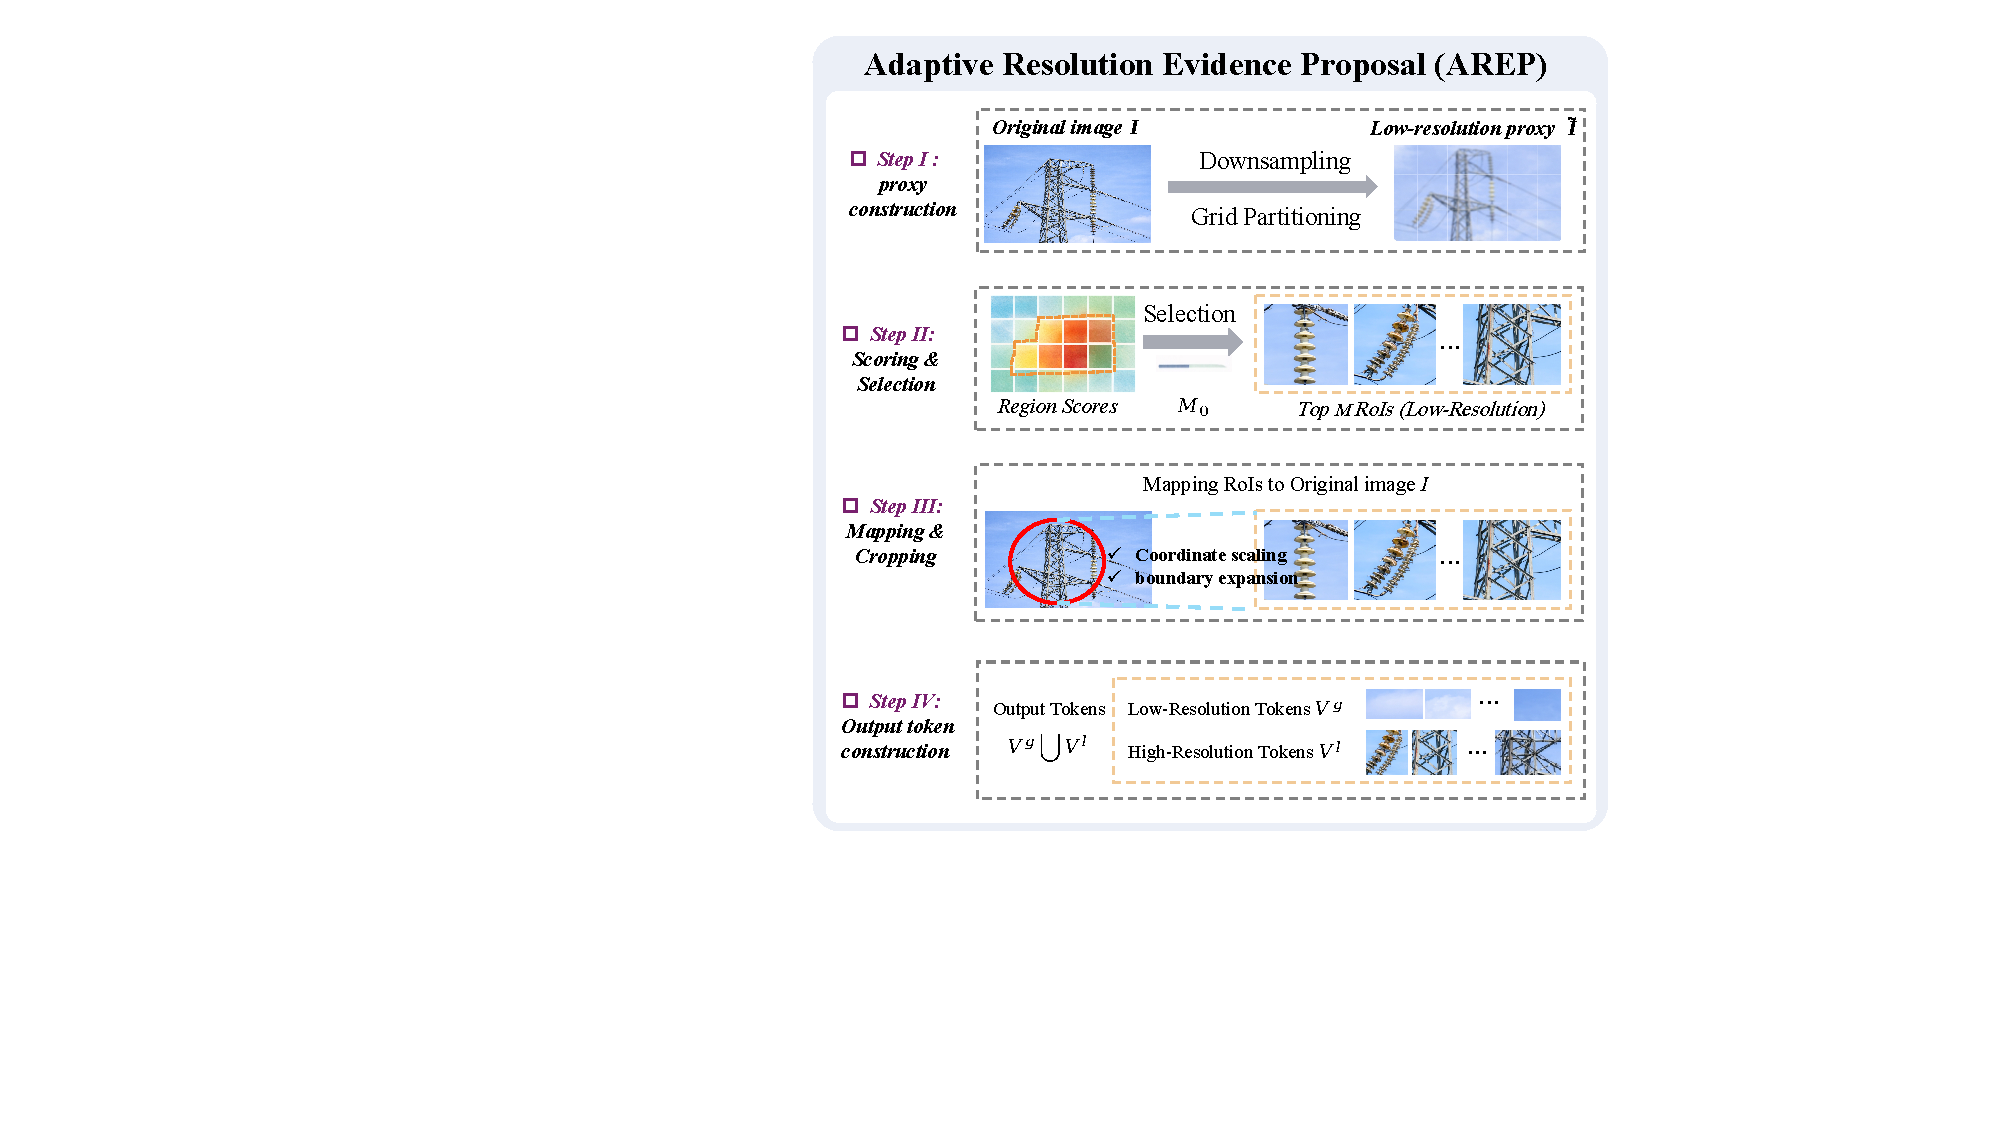
\includegraphics[width=0.98\columnwidth]{AREP.pdf}
  \caption{Illustration of the proposed Adaptive Resolution Evidence Proposal (AREP) module. A low-resolution proxy branch preserves global context and supports lightweight region scoring, after which the top-ranked regions are mapped back to the original high-resolution image for local refinement. The global and local visual tokens are finally concatenated to form the multi-resolution representation delivered to CTS.}
  \label{fig:arep_module}
\end{figure}

% --------------- AREP第一段
\subsubsection{AREP Formulation}
\label{sec:arep_formulation}

Given a high-resolution image $I \in \mathbb{R}^{H \times W \times 3}$, AREP is formulated through four explicit operations: proxy construction, candidate-region generation, proxy-to-original mapping, and budgeted region selection.

First, a low-cost proxy image is constructed as Eq.~\eqref{eq:proxy}
\begin{equation}
  \tilde I = \mathcal{D}(I), \qquad \tilde I\in\mathbb{R}^{\tilde H\times\tilde W\times 3},
  \label{eq:proxy}
\end{equation}
where $\mathcal{D}(\cdot)$ denotes a downsampling operator.
The proxy image is partitioned into $M_0$ candidate regions:
\begin{equation}
  \mathcal{P}=\{P_m\}_{m=1}^{M_0}.
\end{equation}
Each $P_m$ is defined in proxy coordinates and corresponds to a high-resolution crop in the original image through coordinate scaling and boundary expansion.
Let the scale factors be $s_h=H/\tilde H$ and $s_w=W/\tilde W$.
For each candidate region, we define
\begin{equation}
  B_m=\mathcal{W}(P_m; s_h,s_w,\epsilon),
  \label{eq:arep_mapping}
\end{equation}
where $\mathcal{W}(\cdot)$ maps $P_m$ to the original image and expands its boundary by ratio $\epsilon$.

Second, each candidate region is assigned an importance score
\begin{equation}
  g(P_m \mid \tilde I)\in\mathbb{R}_{+},
\end{equation}
and an estimated visual cost $c_m$.
In implementation, $c_m$ corresponds to the token/computation cost of encoding the resized crop from $B_m$.
Let $z_m\in\{0,1\}$ denote whether region $m$ is selected.
AREP is then written as the budget-constrained selection problem
\begin{equation}
  \max_{\{z_m\}_{m=1}^{M_0}}
  \sum_{m=1}^{M_0} z_m\, g(P_m \mid \tilde I)
  \quad
  \mathrm{s.t.}
  \quad
  \sum_{m=1}^{M_0} z_m\, c_m \le \tau_{\mathrm{vis}}.
  \label{eq:arep_budget}
\end{equation}
This objective states that AREP should maximize retained evidence value under a fixed visual budget.
When all selected crops are resized to the same canonical resolution, $c_m$ is approximately constant and Eq.~\eqref{eq:arep_budget} reduces to selecting top-scoring regions under a crop-count budget, which directly matches the practical Top-$M$ procedure in \secref{sec:arep_solution}.

% ------- AREP 第二段
\subsubsection{Practical Solution via Budgeted Foveated Approximation}
\label{sec:arep_solution}

Directly solving Eq.~\eqref{eq:arep_budget} for fine-grained region-level allocation is unnecessary for practical deployment, as a coarse budgeted approximation is sufficient to preserve critical evidence while avoiding the overhead of exact region-wise optimization.
Instead, we adopt a budgeted foveated approximation with two stages: a global low-resolution pass for preserving scene-level context, followed by a small number of local high-resolution refinements for recovering fine-grained evidence.

In practical deployment, we directly reuse the proxy image and candidate-region set defined in \secref{sec:arep_formulation}, rather than restating the full construction.
The proxy branch plays two roles simultaneously: (i) providing a low-cost global representation for scene-level context, and (ii) supporting lightweight region scoring before expensive high-resolution refinement is triggered.

For each candidate region $P_m$, we compute a heuristic importance score on the proxy image.
In the current implementation, the score is defined by the average structural energy within the region:
\begin{equation}
  g(P_m \mid \tilde I)
  =
  \frac{1}{|P_m|}
  \sum_{(x,y)\in P_m}
  \|\nabla \tilde I(x,y)\|_2^2,
  \label{eq:gm}
\end{equation}
where $\nabla \tilde I(x,y)$ denotes the image gradient at location $(x,y)$, and $|P_m|$ is the number of pixels in region $P_m$.
This score favors regions with rich local structures while suppressing visually smooth background areas, thereby providing a lightweight proxy for visual evidence density.

Based on the regional scores $\{g(P_m\mid \tilde I)\}_{m=1}^{M_0}$, the candidate regions are ranked in descending order, and the top-$M$ regions are retained under a predefined crop budget:
\begin{equation}
  \mathcal{R}=\operatorname{TopM}\Big(\{g(P_m\mid \tilde I)\}_{m=1}^{M_0}\Big),
  \label{eq:topm}
\end{equation}
where $\mathcal{R}$ denotes the set of selected regions.
Each selected region is then mapped back to the original image and expanded by a margin ratio $\epsilon$ to conservatively preserve local context and avoid truncating evidence near region boundaries.

AREP maintains a global low-resolution branch and a local high-resolution refinement branch.
The global branch encodes the proxy image as
\begin{equation}
  V^{g}=\phi(\tilde I),
  \label{eq:vg}
\end{equation}
which serves as a compact scene-level representation.
For each refined region $R_j\in\mathcal{R}$, the corresponding image crop is resized to a canonical high-resolution scale and encoded by the vision encoder.
This yields the local token sequence
\begin{equation}
  V^{l}=\operatorname{Concat}\big(\{\phi(I_{R_j})\}_{j=1}^{|\mathcal{R}|}\big),
  \label{eq:vl}
\end{equation}
where $I_{R_j}$ denotes the resized crop associated with region $R_j$.
Finally, the AREP output is formed as
\begin{equation}
  V_{\mathrm{are}}=\operatorname{Concat}(V^{g},V^{l}),
  \label{eq:vare_final}
\end{equation}
which is subsequently passed to CTS for query-conditioned token selection.
Algorithm~\ref{alg:arep} summarizes the overall procedure.

\begin{algorithm}[t]
  \caption{Adaptive Resolution Evidence Proposal (AREP)}
  \label{alg:arep}
  \begin{algorithmic}[1]
    \Require High-resolution image $I$; candidate region set $\mathcal{P}=\{P_m\}_{m=1}^{M_0}$ on the proxy image; crop budget $M$; expansion ratio $\epsilon$
    \Ensure Multi-resolution visual representation $V_{\mathrm{are}}$; selected region set $\mathcal{R}$

    \State Construct proxy image $\tilde I \gets \mathcal{D}(I)$
    \State Obtain global low-resolution tokens $V^{g} \gets \phi(\tilde I)$
    \For{each candidate region $P_m \in \mathcal{P}$}
    \State Compute structural-energy score $g_m \gets g(P_m \mid \tilde I)$
    \EndFor
    \State Rank $\{P_m\}_{m=1}^{M_0}$ in descending order of $\{g_m\}_{m=1}^{M_0}$
    \State Select the top-$M$ regions to form $\mathcal{R}$
    \State Initialize $V^{l} \gets \emptyset$
    \For{each selected region $R_j \in \mathcal{R}$}
    \State Map $R_j$ from proxy coordinates to the original image
    \State Expand $R_j$ by margin ratio $\epsilon$
    \State Crop the corresponding image patch from $I$
    \State Resize the crop to short-side $S_{\mathrm{high}}$ to obtain $I_{R_j}$
    \State Update $V^{l} \gets \operatorname{Concat}(V^{l}, \phi(I_{R_j}))$
    \EndFor
    \State Set $V_{\mathrm{are}} \gets \operatorname{Concat}(V^{g}, V^{l})$
    \State \Return $V_{\mathrm{are}}, \mathcal{R}$
  \end{algorithmic}
\end{algorithm}

\subsubsection{Complexity and Deployment Considerations}
\label{sec:arep_complexity}

AREP is designed as a lightweight front-end evidence proposal module for deployment-oriented high-resolution inspection.
Its practical cost is characterized from three complementary aspects.

First, we define the \emph{AREP overhead} as the additional front-end inference time introduced by proxy construction, regional scoring, ranking, and crop refinement:
\begin{equation}
  T_{\mathrm{AREP}}
  =
  T_{\mathrm{proxy}}
  +
  T_{\mathrm{score}}
  +
  T_{\mathrm{select}}
  +
  T_{\mathrm{crop}}.
  \label{eq:t_arep}
\end{equation}

Second, we characterize the \emph{effective visual computation cost} by the visual tokens retained after AREP, written as
\begin{equation}
  C_{\mathrm{vis}} = |V_{\mathrm{are}}|,
  \label{eq:c_vis}
\end{equation}
which is equivalently controlled in practice by the crop budget $M$ and the resolution of selected local regions.

Third, from a system-level deployment perspective, we report the end-to-end latency and peak GPU memory usage:
\begin{equation}
  (T_{\mathrm{e2e}},\, M_{\mathrm{peak}}),
  \label{eq:deploy_metrics}
\end{equation}
which directly reflect practical feasibility in industrial scenarios.

These metrics provide a unified basis for evaluating whether the visual evidence preserved by AREP justifies its additional front-end cost. The corresponding quantitative results are reported in Sec.~\ref{sec:experiments}.

% ------------- 这里是AREP内容的结束

\begin{figure*}[!t]
  \centering
  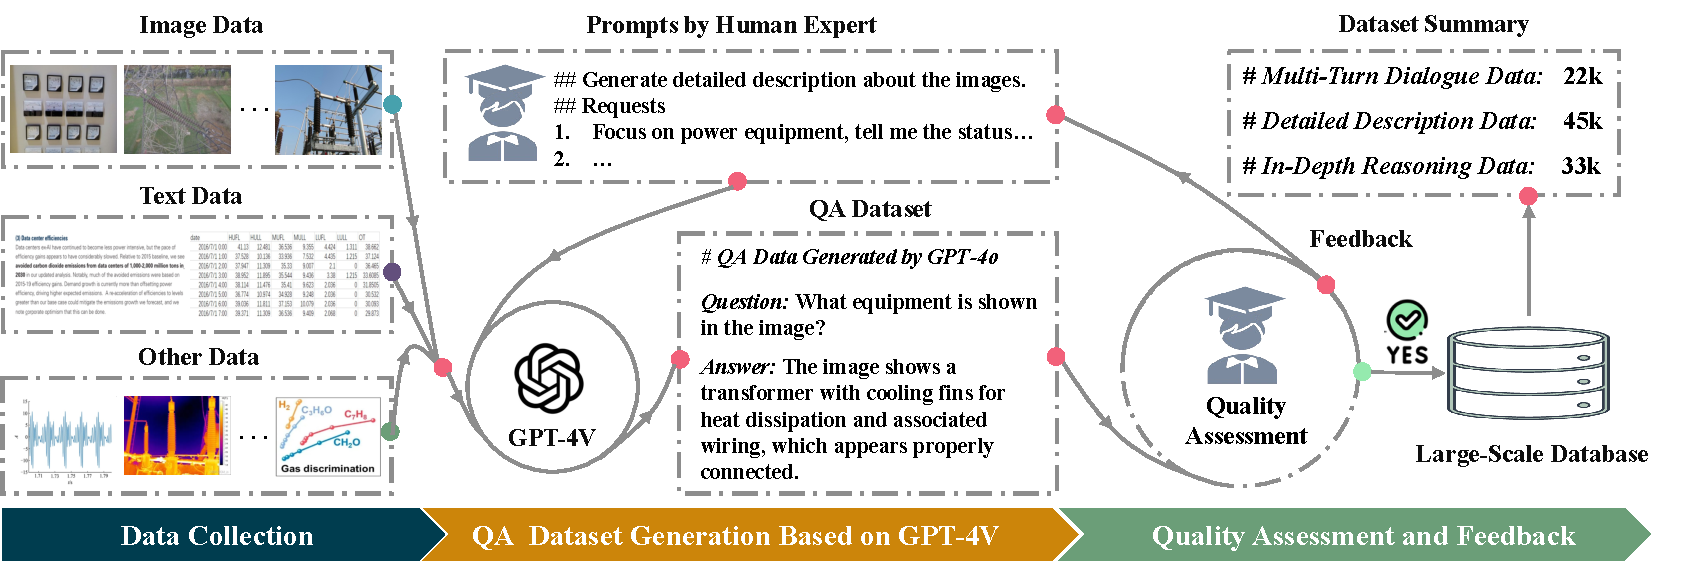
\includegraphics[width=\textwidth]{data_gen.pdf}
  \caption{Overview of the power-oriented instruction data construction pipeline.}
  \label{fig:data_pipeline}
\end{figure*}

\subsection{Coverage-Aware Token Selection (CTS)}
\label{sec:cts}

While AREP performs query-agnostic evidence allocation at the image level, the resulting multi-resolution token stream may still contain substantial redundancy for downstream reasoning. CTS therefore acts as a second-stage, query-conditioned selector at the token level. Given a user instruction and AREP output $V_{\mathrm{are}}$, CTS aims to keep only a compact subset of tokens that preserves both (i) semantic relevance to the query and (ii) spatial continuity along elongated power assets.

\subsubsection{CTS Formulation}
\label{sec:cts_formulation}

Let the AREP output be
\[
  V_{\mathrm{are}}=\{v_i\}_{i=1}^{N},
\]
where each token $v_i$ is associated with a spatial coordinate $p_i\in\mathbb{R}^2$ on the image plane (obtained by mapping patch/crop locations back to image coordinates).
For local-crop tokens, patch coordinates are first defined in crop space and then mapped back to the original image plane through the crop-to-image transform, so that global and local tokens share a common spatial reference.
Given the query token sequence $T=\{t_j\}_{j=1}^{M}$, we aggregate query-to-vision cross-attention as
\begin{equation}
  A_{j,i}=\frac{1}{|\mathcal{L}_a|\,H}
  \sum_{\ell\in\mathcal{L}_a}\sum_{h=1}^{H}
  \operatorname{Attn}^{(\ell,h)}(t_j\!\rightarrow\! v_i),
  \label{eq:cts_attn}
\end{equation}
where $\mathcal{L}_a$ is a selected set of upper multimodal layers and $H$ is the number of attention heads.
In practice, these attention signals are extracted from a lightweight multimodal scoring pass over the AREP-compressed token stream, after which only the selected subset is retained for subsequent answer generation.
The token importance score is then defined as
\begin{equation}
  s_i=\sum_{j=1}^{M} w_j A_{j,i},
  \qquad w_j\ge 0,\ \sum_{j=1}^{M}w_j=1,
  \label{eq:cts_score}
\end{equation}
with uniform $w_j=1/M$ in our default setting.

To encode continuity, CTS partitions tokens into ordered strips along a principal axis $u\in\mathbb{R}^2$ (estimated from token coordinates by PCA):
\begin{equation}
  \begin{aligned}
    r_i &= u^\top p_i,\\
    \Delta &= \frac{r_{\max}-r_{\min}}{B},\\
    \Omega_b &= \Big\{i\ \big|\ r_i\in\left[r_{\min}+(b-1)\Delta,\ r_{\min}+b\Delta\right)\Big\},\\
    &\qquad b=1,\ldots,B.
  \end{aligned}
  \label{eq:cts_partition}
\end{equation}
When the token layout does not exhibit a stable dominant direction, CTS falls back to a default horizontal image axis, thereby degenerating to coverage-aware spatial sampling instead of relying on a line-specific prior.
Let $z_i\in\{0,1\}$ denote whether token $v_i$ is selected. CTS is formulated as
\begin{equation}
  \begin{aligned}
    \max_{\{z_i\}_{i=1}^{N}}\quad
    &\sum_{i=1}^{N} z_i\, s_i,\\
    \mathrm{s.t.}\quad
    &\sum_{i=1}^{N} z_i \le K,\\
    &\sum_{i\in\Omega_b} z_i \ge k_b,\qquad b=1,\ldots,B.
  \end{aligned}
  \label{eq:cts_opt}
\end{equation}
with feasibility condition $\sum_{b=1}^{B}k_b\le K$.
The final CTS output is
\begin{equation}
  V_{\mathrm{cts}}=\{v_i\in V_{\mathrm{are}}\mid z_i=1\},
  \label{eq:vcts}
\end{equation}
which is passed to the MLLM for answer generation.

\subsubsection{Practical Solution Algorithm}
\label{sec:cts_solution}

Directly solving the discrete problem in \eqnref{eq:cts_opt} is unnecessary in practice.
We therefore adopt a lightweight two-stage greedy approximation that enforces coverage first and fills the remaining budget by global relevance.

First, we compute relevance scores $\{s_i\}$ using \eqnref{eq:cts_attn} and \eqnref{eq:cts_score}, and build strips $\{\Omega_b\}$ via \eqnref{eq:cts_partition}.
Then, CTS performs coverage-aware selection in two stages:
\begin{equation}
  \begin{aligned}
    \mathcal{S}_b
    &= \operatorname{Top}_{\min(k_b,|\Omega_b|)}\big(\{s_i\mid i\in\Omega_b\}\big),\\
    &\qquad b=1,\ldots,B,\\
    \mathcal{S}
    &= \bigcup_{b=1}^{B}\mathcal{S}_b,\\
    \bar{\mathcal{S}}
    &= \{1,\ldots,N\}\setminus\mathcal{S},\\
    \hat{\mathcal{S}}
    &= \operatorname{Top}_{K-|\mathcal{S}|}\big(\{s_i\mid i\in\bar{\mathcal{S}}\}\big).
  \end{aligned}
  \label{eq:cts_stage}
\end{equation}
Finally, $\mathcal{S}\leftarrow\mathcal{S}\cup\hat{\mathcal{S}}$, and the selected tokens are returned as
\begin{equation}
  V_{\mathrm{cts}}=\{v_i\in V_{\mathrm{are}}\mid i\in\mathcal{S}\}.
  \label{eq:vcts_sol}
\end{equation}
This procedure has complexity dominated by sorting (approximately $O(N\log N)$), making CTS suitable for real-time deployment.
Algorithm~\ref{alg:cts} summarizes the complete process.

\begin{algorithm}[t]
  \caption{Coverage-Aware Token Selection (CTS)}
  \label{alg:cts}
  \begin{algorithmic}[1]
    \Require AREP tokens $V_{\mathrm{are}}=\{v_i,p_i\}_{i=1}^{N}$; query tokens $T=\{t_j\}_{j=1}^{M}$; budget $K$; strip number $B$; strip quotas $\{k_b\}_{b=1}^{B}$
    \Ensure Selected token subset $V_{\mathrm{cts}}$

    \State Compute aggregated attention $A$ by \eqnref{eq:cts_attn}
    \State Compute token scores $s_i$ by \eqnref{eq:cts_score}
    \State Estimate principal axis $u$ from $\{p_i\}_{i=1}^{N}$ and build strips $\{\Omega_b\}_{b=1}^{B}$ by \eqnref{eq:cts_partition}
    \State Initialize $\mathcal{S}\gets\emptyset$
    \For{$b=1$ to $B$}
    \State Select $\mathcal{S}_b\gets \operatorname{Top}_{\min(k_b,|\Omega_b|)}(\{s_i\mid i\in\Omega_b\})$
    \State Update $\mathcal{S}\gets\mathcal{S}\cup\mathcal{S}_b$
    \EndFor
    \State Set $\bar{\mathcal{S}}\gets\{1,\ldots,N\}\setminus\mathcal{S}$
    \State Select $\hat{\mathcal{S}}\gets \operatorname{Top}_{K-|\mathcal{S}|}(\{s_i\mid i\in\bar{\mathcal{S}}\})$
    \State Update $\mathcal{S}\gets\mathcal{S}\cup\hat{\mathcal{S}}$
    \State Set $V_{\mathrm{cts}}\gets\{v_i\in V_{\mathrm{are}}\mid i\in\mathcal{S}\}$
    \State \Return $V_{\mathrm{cts}}$
  \end{algorithmic}
\end{algorithm}

\section{Domain Adaptation and Knowledge Augmentation}
\label{sec:domain_adapt}

While Section~\ref{sec:method} focuses on efficient evidence mining for high-resolution power VQA, achieving domain-correct and reliable responses further requires adapting the foundation MLLM to power-system terminology, task formats, and operational knowledge. To this end, we construct power-oriented instruction data from real monitoring scenarios and perform supervised instruction tuning on an open-source MLLM. Moreover, we integrate citation-grounded retrieval-augmented generation (RAG) to incorporate power regulations and defect criteria, enabling traceable knowledge grounding in the generated answers.

\subsection{Power-Oriented Instruction Data Construction}
\label{sec:data_construction}
As illustrated in Fig.~\ref{fig:data_pipeline}, we construct the power-oriented instruction corpus through a lightweight semi-automatic pipeline. We first collect heterogeneous sources, including monitoring images, textual materials, and auxiliary data, and then use expert-designed prompts to guide GPT-4V/GPT-4o for data generation. A subsequent quality-assessment and feedback stage is applied to filter noisy outputs and refine the generated samples. The final corpus is organized into image--instruction--response triplets for downstream instruction tuning. The composition of the corpus is summarized in Table~\ref{tab:instruction_stats}.

\begin{table}[!b]
  \centering
  \caption{Composition of the power-oriented instruction corpus used for SFT.}
  \label{tab:instruction_stats}
  \footnotesize
  \setlength{\tabcolsep}{0pt}
  \renewcommand{\arraystretch}{1.12}
  \begin{tabular*}{\columnwidth}{@{\extracolsep{\fill}}>{\raggedright\arraybackslash}m{1.76cm}>{\raggedright\arraybackslash}m{4.48cm}>{\centering\arraybackslash}m{0.78cm}@{}}
    \toprule
    Subset & Main supervision focus & \#Inst. \\
    \midrule
    \makecell[l]{Detailed\\descriptions} & Fine-grained visual grounding of equipment, states, and spatial relations & 45k \\
    \addlinespace[0.5ex]
    \makecell[l]{Multi-turn\\dialogues} & Context-aware interaction across consecutive user queries & 22k \\
    \addlinespace[0.5ex]
    \makecell[l]{In-depth\\reasoning/QA} & Evidence-to-decision supervision for diagnosis, severity assessment, and O\&M recommendation & 33k \\
    \midrule
    Total & -- & 100k \\
    \bottomrule
  \end{tabular*}
\end{table}

\subsection{Domain Adaptation via Supervised Instruction Tuning}
\label{sec:sft}
We instantiate domain adaptation on the Qwen3-VL-4B backbone and fine-tune it on the power-oriented image--instruction--response triplets constructed in Sec.~\ref{sec:data_construction}. For each training sample, the image and instruction are provided as the condition, and the model is optimized with teacher forcing to maximize the likelihood of the target response. We keep the prompt format consistent with downstream inference so that the learned behavior transfers directly to deployment-time VQA. This stage injects power-domain terminology, question formats, and answer patterns into the model parameters; the exact optimizer and schedule are reported in Sec.~\ref{sec:exp_settings}.

\subsection{Knowledge Augmentation with Citation-Grounded RAG}
\label{sec:rag}
To further improve correctness on regulation-sensitive questions, we build a power-domain knowledge base from regulations, defect criteria, and handling guidelines. At inference time, the current query is used to retrieve a small set of relevant passages, which are inserted into the prompt as indexed evidence snippets together with the image and question. The MLLM is then instructed to generate its answer by grounding the judgment on the retrieved evidence and to return the corresponding citation indices. As a result, the final response is not only more accurate but also auditable, because the answer can be traced back to the exact evidence presented to the model.

\begin{table*}[t]
  \centering
  \caption{Overall benchmark performance and deployment-oriented efficiency. \emph{Latency} is measured as end-to-end time per question (ms/q) on a single NVIDIA A100 GPU using BF16 precision; \emph{Tokens} reports effective visual tokens processed by the MLLM (from original $N$ to pruned $K$).}
  \label{tab:main_results}

  % 定义专业学术蓝
  \definecolor{tableblue}{RGB}{232, 240, 250}
  \renewcommand{\arraystretch}{1.3}
  \small
  \setlength{\tabcolsep}{4pt}

  % 使用 tabular* 并设置宽度为 0.95\textwidth，所有列使用 c 居中
  \begin{tabular*}{0.98\textwidth}{@{\extracolsep{\fill}} *{11}{c} @{}}
    \toprule
    \textbf{Model} & \textbf{Type} & \textbf{Params} & \textbf{Acc.} & \textbf{Percep.} & \textbf{Reason.} & \textbf{Action} & \textbf{Latency} & \textbf{Tokens} & \textbf{Peak Mem.} & \textbf{Tag} \\
    & & \textbf{(B)} & \textbf{(\%)} & \textbf{(\%)} & \textbf{(\%)} & \textbf{(\%)} & \textbf{(ms/q)} & \textbf{($N \!\rightarrow\! K$)} & \textbf{(GB)} & \\
    \midrule

    % 闭源模型组 - 加上 @{} 彻底消除色块溢出
    \rowcolor{tableblue} \multicolumn{11}{c}{\textit{Closed-source MLLMs}} \\
    GPT-4o & Closed & -- & 76.1 & 79.4 & 78.5 & 70.4 & -- & -- & -- & API \\
    Gemini-2.5-Pro & Closed & -- & 77.4 & 80.1 & 78.9 & 73.2 & -- & -- & -- & API \\
    \midrule

    % 开源模型组 - 加上 @{} 彻底消除色块溢出
    \rowcolor{tableblue} \multicolumn{11}{c}{\textit{Open-source MLLMs}} \\
    Qwen3-VL-4B & Open & 4.4 & 49.7 & 52.1 & 51.8 & 45.2 & 850 &  4096 & 12.2 & Full-res \\
    Qwen3-VL-8B & Open & 8.2 & 55.3 & 58.7 & 57.3 & 49.9 & 1320 &  4096 & 20.5 & Full-res \\
    InternVL3-4B & Open & 4.2 & 50.2 & 52.6 & 51.9 & 46.1 & 880 &  4096 & 11.9 & Full-res \\
    InternVL3-8B & Open & 7.6 & 57.8 & 59.2 & 58.8 & 55.4 & 1410 &  4096 & 21.2 & Full-res \\
    LLaVA-1.5-8B & Open & 7.8 & 43.3 & 46.4 & 45.7 & 37.8 & 1380 &  4096 & 19.8 & Full-res \\
    \midrule

    % 我们的方案组 - 加上 @{} 彻底消除色块溢出
    \rowcolor{tableblue} \multicolumn{11}{c}{\textit{Ours / Variants (Backbone: Qwen3-VL-4B)}} \\
    \textbf{PowerBrain} & Ours & 4.4 & 73.6 & 76.8 & 75.3 & 68.7 & \textbf{320} & 4096 $\rightarrow$ \textbf{256} & \textbf{8.2} & \textbf{Full} \\
    \quad w/o AREP & Ours & 4.4 & 69.8 & 72.2 & 71.6 & 65.6 & 450 & 4096 $\rightarrow$ 256 & 9.4 & No-ROI \\
    \quad w/o CTS (Top-$K$) & Ours & 4.4 & 70.9 & 73.5 & 72.1 & 67.1 & 315 & 4096 $\rightarrow$ 256 & 8.1 & Top-$K$ \\
    \quad w/o RAG & Ours & 4.4 & 64.2 & 67.8 & 65.6 & 59.2 & 320 & 4096 $\rightarrow$ 256 & 8.2 & No-RAG \\
    \quad w/o SFT & Ours & 4.4 & 66.8 & 69.1 & 67.4 & 63.9 & 320 & 4096 $\rightarrow$ 256 & 8.2 & No-SFT \\
    \midrule

    % 底部注释，左对齐不受影响
    \multicolumn{11}{l}{\scriptsize \textit{Note: Closed-source models were evaluated using the latest available APIs as of December 2025. All tests used BF16 precision.}} \\
    \bottomrule
  \end{tabular*}
\end{table*}

\section{Experiments}
\label{sec:experiments}

The experimental evaluation is organized around four questions. 
\emph{Q1: Diagnostic performance.} 
We examine whether the proposed PowerBrain improves diagnostic accuracy over representative open-source and closed-source MLLMs on high-resolution power inspection VQA. 
\emph{Q2: Deployment efficiency.} 
We evaluate whether the proposed evidence-mining pipeline reduces deployment cost in terms of visual tokens, latency, and peak GPU memory. 
\emph{Q3: Module contribution.} 
We isolate the effects of AREP, CTS, SFT, and RAG through ablation studies. 
\emph{Q4: Generality and interpretability.} 
We assess whether the framework generalizes across multiple power inspection scenarios and produces interpretable evidence traces for auditable O\&M decision support.

\subsection{Experimental Settings}
\label{sec:exp_settings}

PowerBrain is instantiated on the Qwen3-VL-4B backbone~\cite{qwen3} and implemented with PyTorch and Hugging Face Transformers. Supervised instruction tuning is performed on power-oriented image--instruction--response triplets using teacher forcing, where the image and user instruction are used as conditions and the target response is optimized as the supervision signal. Training is conducted on 16 NVIDIA A100 80GB GPUs with BF16 mixed precision and gradient checkpointing. We use AdamW with learning rate $2\times10^{-5}$, weight decay 0.05, global batch size 256, warmup ratio 0.05, and cosine learning-rate decay. The full SFT run takes approximately 12 hours for 3000 update steps.

For comparison, open-source MLLM baselines are evaluated from their official checkpoints without power-domain fine-tuning. All PowerBrain variants share the same Qwen3-VL-4B backbone and differ only in the enabled modules, such as AREP, CTS, SFT, or RAG. For RAG-enabled inference, the retriever returns the top-3 relevant snippets from the power-maintenance knowledge base, which are inserted into the prompt with citation indices.

Unless otherwise stated, AREP uses $S_{\mathrm{low}}=512$, $S_{\mathrm{high}}=1536$, $M=6$, $\epsilon=0.15$, and a $12\times12$ proxy grid. CTS keeps at most $K=256$ visual tokens, with $B=16$ strips and minimum quota $k_b=1$. All token-selection baselines are evaluated under the same token budget $K$.

\subsection{Benchmark and Evaluation Protocol}
\label{sec:benchmark_protocol}


To evaluate both high-resolution evidence mining and cross-scenario task generality, we curate a multi-task benchmark from real-world power monitoring data and O\&M requirements. The benchmark contains 3,290 image-question pairs and covers five representative inspection scenarios: transmission-line foreign-object inspection, disconnect-switch state recognition, meter reading, power-scene safety recognition, and insulator infrared diagnosis. All samples are organized under a unified VQA interface, and the task composition is summarized in Table~\ref{tab:benchmark_tasks}. No evaluation image-question pair is used for supervised instruction tuning.

\begin{table}[!t]
  \centering
  \caption{Composition of the PowerBrain benchmark.}
  \label{tab:benchmark_tasks}
  \footnotesize
  \setlength{\tabcolsep}{2pt}
  \renewcommand{\arraystretch}{1.08}
  \begin{tabular*}{\columnwidth}{@{\extracolsep{\fill}}>{\raggedright\arraybackslash}p{1.45cm}>{\raggedright\arraybackslash}p{1.35cm}>{\centering\arraybackslash}p{0.96cm}>{\raggedright\arraybackslash}p{2.61cm}@{}}
    \toprule
    Sub-task & Image type & \makecell[c]{\#\\Samples} & Main focus \\
    \midrule
    Line foreign object & RGB panorama & xxx & small-object / O\&M decision \\
    Disconnect switch & RGB close-up & xxx & state recognition \\
    Meter reading & RGB close-up & xxx & OCR / reading \\
    Scene safety & RGB worksite & xxx & safety violation \\
    Infrared diagnosis & IR image & xxx & thermal abnormality \\
    \bottomrule
  \end{tabular*}
\end{table}

To enable consistent comparison across heterogeneous tasks, each sample is converted into a single-turn MCQ instance. Each model receives the image, question, and candidate options, and is instructed to output only the option letter. The option order is randomized to mitigate positional bias. The correct option is determined by expert annotation or verified inspection records, and ambiguous samples are removed during quality checking.

We report overall accuracy and PRA-category accuracy. Overall accuracy is computed over all MCQ samples, while Perception, Reasoning, and Action accuracies are computed on their corresponding question subsets. We also report deployment-oriented metrics, including the effective number of visual tokens fed into the MLLM, end-to-end latency, and peak GPU memory. Latency and memory are measured on a single NVIDIA A100 80GB GPU under BF16 precision. For closed-source APIs, only accuracy-related metrics are reported because their serving hardware and memory usage are inaccessible.

In its current split, the benchmark contains 3,290 image-question pairs in total. 
As shown in \figref{fig:resolution_distribution}, the full benchmark exhibits a pronounced long-tail resolution distribution, with a peak resolution of 4896$\times$3968. 
Approximately 45.2\% of the images are no larger than 1080p, 47.5\% fall between 1080p and 4K UHD, and 7.3\% exceed 4K UHD. 
This distribution reflects the practical characteristics of power inspection imagery: many samples are high-resolution monitoring images, while diagnostically relevant evidence often occupies only a small portion of the scene. 
These statistics motivate deployment-oriented evidence mining instead of dense full-image encoding.

\begin{figure}[!t]
  \centering
  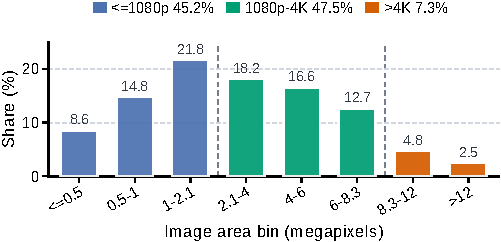
\includegraphics[width=\columnwidth]{resolution_dynamic_size_cloud_regen.pdf}
  \caption{Resolution distribution of the PowerBrain benchmark. The benchmark contains a substantial high-resolution portion: 45.2\% of images are no larger than 1080p, 47.5\% fall between 1080p and 4K UHD, and 7.3\% exceed 4K UHD, with a peak resolution of 4896$\times$3968.}
  \label{fig:resolution_distribution}
\end{figure}

\subsection{Main Results and Efficiency}
\label{sec:main_results_efficiency}

Table~\ref{tab:main_results} answers Q1 and Q2 by comparing PowerBrain with representative closed-source APIs, open-source MLLMs, and ablated variants under the same benchmark protocol. We discuss the results from two perspectives: diagnostic performance and deployment-oriented efficiency.

\subsubsection{Overall Diagnostic Performance}
PowerBrain attains \textbf{73.6\%} overall accuracy on the benchmark, substantially outperforming open-source baselines of similar scale. Relative to the vanilla Qwen3-VL-4B, which uses the same 4.4B backbone, the gain is \textbf{+23.9} percentage points (73.6\% vs. 49.7\%). PowerBrain also exceeds larger 8B open-source models, improving over InternVL3-8B by \textbf{+15.8} points and over LLaVA-1.5-8B by \textbf{+30.3} points. 
These results indicate that domain adaptation and evidence selection provide substantial gains beyond simply increasing model scale in this benchmark.

Compared with closed-source APIs, PowerBrain remains competitive despite its much smaller model size. The gap to GPT-4o and Gemini-2.5-Pro is limited to 2.5--3.8 percentage points in overall accuracy, while the \textit{Action} metric reaches \textbf{68.7\%}, close to GPT-4o (\textbf{70.4\%}). This behavior is important for industrial deployment: generalized MLLMs may recognize visual content reasonably well, but actionable O\&M decisions require domain-aligned reasoning and regulation-aware judgment, which are directly strengthened by SFT and citation-grounded RAG.

\subsubsection{Deployment-Oriented Efficiency}
The accuracy gains are obtained together with a substantial reduction in inference cost. PowerBrain reduces the effective visual token budget from \textbf{4096} to \textbf{256}, corresponding to a \textbf{93.7\%} reduction in visual tokens processed by the MLLM. This compression directly translates into lower resource consumption: peak GPU memory decreases from 12.2 GB for Qwen3-VL-4B to \textbf{8.2 GB}, i.e., a \textbf{32.7\%} reduction.

Latency shows a similar trend. PowerBrain requires \textbf{320 ms/q}, compared with 850 ms/q for Qwen3-VL-4B and 1410 ms/q for InternVL3-8B, corresponding to speedups of \textbf{2.65$\times$} and \textbf{4.4$\times$}, respectively. Taken together, the results in Table \ref{tab:main_results} show that the proposed evidence-mining pipeline improves the accuracy--efficiency trade-off rather than merely shifting it, which is essential for UAV- or substation-oriented deployment under limited memory and response-time budgets.

\subsection{Ablation and Scaling Analysis}
\label{sec:ablation_scaling}

To answer Q3, we conduct ablation studies on the key components of PowerBrain under the same evaluation protocol. 
The analysis focuses on two evidence-mining modules: AREP, which determines where high-resolution visual budgets are allocated at the image level, and CTS, which determines which visual tokens are retained under a fixed token budget. 
We further discuss the effects of SFT and citation-grounded RAG using the variants reported in Table~\ref{tab:main_results}. 
For key paired comparisons, statistical significance is assessed using McNemar's test on MCQ predictions, and bootstrap confidence intervals are reported where applicable.

\subsubsection{AREP: Proposal Strategy and Micro-Evidence Preservation}
\label{sec:ablation_arep}

AREP is designed to preserve micro-scale evidence by allocating high-resolution crops to informative regions. 
To examine whether the proposed structural-energy score provides effective region prioritization, we compare several proposal strategies under the same crop budget $M$ and the same downstream CTS configuration. 
The compared variants include random ROI selection, uniform ROI selection, edge-density-based proposal, and the proposed gradient-energy AREP. 
The w/o AREP variant removes local high-resolution refinement and degrades to global low-resolution encoding.

Table~\ref{tab:arep_strategy_ablation} reports the results. 
Besides overall accuracy, we report Micro Acc. on the micro-evidence subset and ROI Hit@M on annotated samples. 
For a sample with annotated evidence region $B_n$ and selected ROI set $\mathcal{R}_n$, ROI Hit@M is computed as
\begin{equation}
\mathrm{Hit@M}
=
\frac{1}{N}
\sum_{n=1}^{N}
\mathbf{1}
\left[
\max_{R_j\in\mathcal{R}_n}
\frac{|R_j\cap B_n|}{|B_n|}
>
\eta
\right],
\label{eq:hitm}
\end{equation}
where $\eta$ is the coverage threshold. 
This metric evaluates whether the selected high-resolution regions actually cover task-critical evidence, rather than only improving the final answer indirectly.

As shown in Table~\ref{tab:arep_strategy_ablation}, Gradient-energy AREP achieves the highest overall accuracy of XX.X\% and Micro Acc. of XX.X\%, outperforming Random ROI and Uniform ROI by XX.X and XX.X percentage points on the micro-evidence subset, respectively. 
It also obtains the highest ROI Hit@M of XX.X\%, indicating that the selected regions more reliably cover task-critical evidence. 
Compared with edge-density proposal, Gradient-energy AREP provides a better balance between evidence coverage and computational cost, while introducing only XX ms/q of additional latency.


\begin{table}[t]
  \centering
  \caption{Ablation of AREP proposal strategies under the same crop budget $M$.}
  \label{tab:arep_strategy_ablation}
  \footnotesize
  \setlength{\tabcolsep}{0pt}
  \renewcommand{\arraystretch}{1.05}
  \begin{tabular*}{\columnwidth}{@{\extracolsep{\fill}}lcccc@{}}
  \toprule
  Proposal strategy & Acc. & Micro Acc. & ROI Hit@M & Latency \\
  & (\%) & (\%) & (\%) & (ms/q) \\
  \midrule
  w/o AREP              & -- & -- & N/A & -- \\
  Random ROI            & -- & -- & --  & -- \\
  Uniform ROI           & -- & -- & --  & -- \\
  Edge-density ROI      & -- & -- & --  & -- \\
  Gradient-energy AREP  & -- & -- & --  & -- \\
  \bottomrule
  \end{tabular*}
\end{table}



\subsubsection{CTS: Selection Strategy and Token-Budget Sensitivity}
\label{sec:ablation_cts}

CTS aims to retain query-relevant visual tokens while preserving the continuity of structured evidence. 
We compare CTS with random selection, uniform sampling, and attention-based Top-K selection under the same token budget $K=256$. 
Table~\ref{tab:cts_strategy_ablation} summarizes the results. 
We further vary $K$ to evaluate the token-budget sensitivity under tighter and looser visual-token budgets.


\begin{table}[t]
  \centering
  \caption{Ablation of token selection strategies under the same token budget $K=256$.}
  \label{tab:cts_strategy_ablation}
  \footnotesize
  \setlength{\tabcolsep}{0pt}
  \renewcommand{\arraystretch}{1.05}
  \begin{tabular*}{\columnwidth}{@{\extracolsep{\fill}}lccccc@{}}
  \toprule
  Selection strategy & Query score & Coverage & Acc. & Action & StripCov \\
  &  &  & (\%) & (\%) & (\%) \\
  \midrule
  Random & -- & -- & -- & -- & -- \\
  Uniform & -- & weak & -- & -- & -- \\
  Attention Top-K & \checkmark & -- & -- & -- & -- \\
  CTS & \checkmark & \checkmark & -- & -- & -- \\
  \bottomrule
  \end{tabular*}
\end{table}


\subsubsection{Domain Adaptation and Knowledge Grounding}
\label{sec:ablation_sft_rag}

Finally, we examine the contributions of supervised instruction tuning and citation-grounded retrieval using the ablated variants in Table~\ref{tab:main_results}. 
Removing SFT decreases the overall accuracy from 73.6\% to 66.8\%, indicating that domain-oriented instruction tuning is important for adapting the backbone to power-specific terminology, question formats, and response patterns. 
Removing RAG leads to a larger drop in the Action metric, from 68.7\% to 59.2\%, suggesting that retrieved maintenance regulations and defect-handling guidelines are particularly useful for O\&M-oriented decision support.





\lmx{Above is the new version of ablation}


\subsection{Case Studies and Explainability}
\label{sec:case_studies}

We provide qualitative case studies to illustrate how the proposed framework produces accurate and auditable answers under challenging high-resolution power inspection scenarios.
Our explainability is grounded on two exported evidence layers: (i) corridor-level ROIs proposed by AREP, and (ii) token-level saliency/selection maps produced by CTS, which can be projected back to image patches to visualize what the model attends to.

\begin{figure*}[!t]
  \centering
  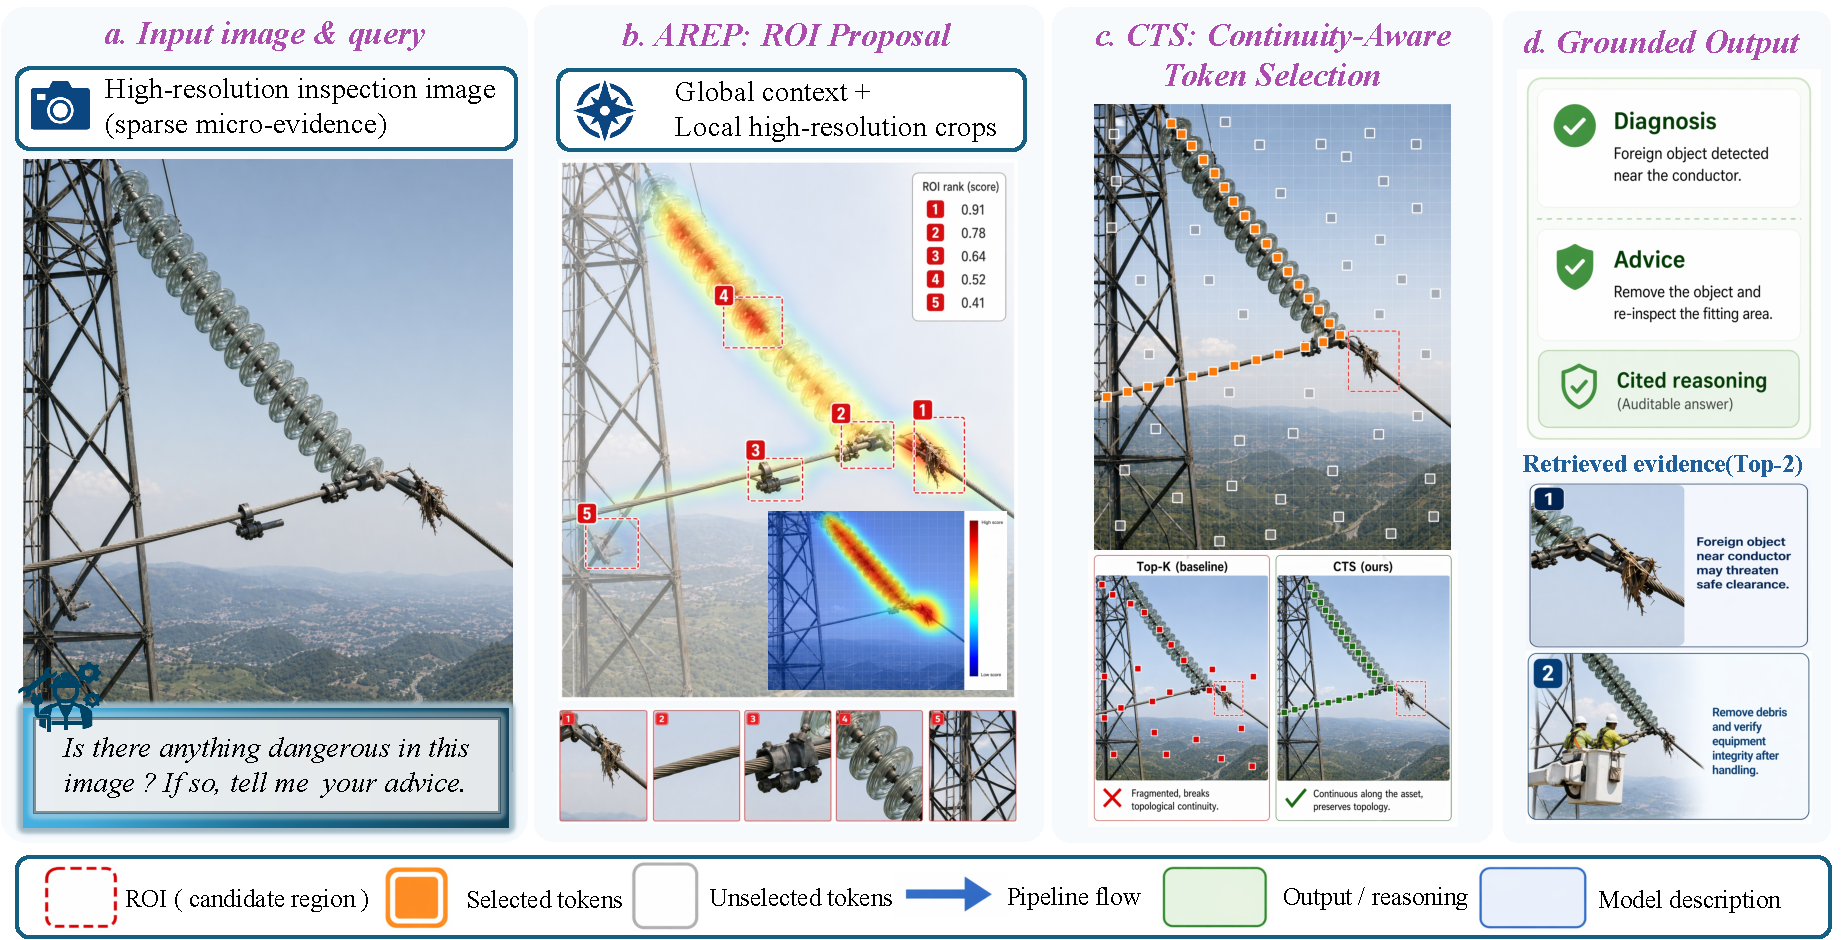
\includegraphics[width=0.98\textwidth]{case_study.pdf}
  \caption{Visualization of the PowerBrain pipeline on a representative high-resolution inspection case. Given a corridor-scale image and a user query, AREP first proposes high-value ROIs from a low-resolution proxy, CTS then retains a compact yet topologically coherent set of query-relevant tokens, and the final answer is grounded with retrieved domain evidence to support auditable diagnosis and maintenance advice.}
  \label{fig:case_example}
\end{figure*}

\subsubsection{Pipeline example with grounded evidence flow.}
Fig.~\ref{fig:case_example} visualizes the end-to-end decision process of PowerBrain on a representative high-resolution inspection case.
Starting from the input image and query, AREP first identifies structurally informative ROIs, after which CTS preserves a compact yet continuous set of query-relevant tokens for multimodal reasoning.
The final response is further grounded with retrieved domain evidence, producing an auditable diagnosis and maintenance suggestion.
This example qualitatively illustrates how PowerBrain couples fine-grained visual evidence preservation with citation-grounded reasoning in safety-critical power inspection scenarios.

\subsubsection{Evidence localization via ROI and token-level maps.}
To make the decision process auditable, we visualize the corridor ROIs and token-level evidence maps for representative queries.
AREP suppresses dominant background regions and focuses computation on physically plausible conductor corridors, whereas CTS further highlights query-relevant tokens within the corridor (e.g., fittings, insulators, foreign objects) and preserves continuity along the conductor direction.
In contrast, Top-\(K\) selection often yields fragmented evidence concentrated in a local area, which can lead to unstable reasoning on elongated targets.
These visualizations provide an intuitive explanation of why coverage-aware selection improves execution-oriented decisions and reduces attention drift.

\subsubsection{Citation-grounded reasoning with RAG.}
For safety-critical queries that require adherence to operational regulations, we additionally display retrieved textual evidence and the corresponding citations used in the final response.
RAG encourages the model to ground its recommendations on explicit rules or defect-handling guidelines, improving both correctness and traceability.
We observe that the grounded answers are more consistent across paraphrased queries and option shuffles, which is essential for online O\&M decision support.

\section{Conclusion and Discussion}
\label{sec:conclusion}

This paper investigated efficient and explainable high-resolution VQA for power inspection with a domain-adapted multimodal large language model.
Motivated by the characteristics of real-world power monitoring imagery---\emph{high resolution, dominant background redundancy, and sparse/elongated evidence along transmission corridors}---we developed a coarse-to-fine evidence mining framework that enables deployment-oriented inference under constrained computation budgets.

Specifically, we proposed a recall-oriented adaptive-resolution evidence proposal (AREP) module to suppress irrelevant background and provide corridor-level evidence candidates, and a coverage-aware instruction-guided token selection (CTS) module to select query-relevant visual tokens under a token budget while preserving evidence continuity for thin and elongated targets.
To improve domain correctness and auditability, we further performed supervised instruction tuning (SFT) on power-oriented instruction data and integrated citation-grounded retrieval-augmented generation (RAG) with power regulations and defect-handling knowledge, enabling traceable and professional responses in safety-critical scenarios.

Extensive experiments on a multi-task benchmark covering transmission-line inspection, disconnect-switch state recognition, meter OCR, safety recognition, and insulator infrared diagnosis demonstrated that the proposed system achieves a favorable performance--efficiency trade-off.
In particular, the evidence mining pipeline substantially reduces effective visual token consumption and deployment costs (latency and memory) without sacrificing accuracy, while ablation and scaling analyses verified the functional roles of AREP, continuity-aware selection, SFT, and RAG.
Qualitative case studies further illustrated that the exported ROI- and token-level evidence maps, together with citation-grounded reasoning, support explainable and auditable inspection results.

There remain several directions for future work.
First, while AREP and CTS are designed for conservative evidence recall and continuity, further improving robustness under severe adverse conditions (e.g., heavy occlusion, extreme illumination, and motion blur) is of practical interest, potentially by incorporating adaptive fallback strategies and uncertainty-aware evidence selection.
Second, expanding the knowledge base and maintaining up-to-date regulations and defect criteria are important for long-term deployment; systematic methods for knowledge curation, validation, and conflict resolution will further enhance reliability.
Third, extending the framework to broader power inspection tasks with richer modalities (e.g., video streams, thermal sequences, and multi-sensor time series) and studying continual adaptation across sites and devices are promising directions toward scalable industrial applications.

\bibliographystyle{IEEEtran}
\bibliography{refs}

\end{document}
